% Skrivet av Nils

\usetikzlibrary{shapes,backgrounds}

\def\rad{1.5}
\def\dcircle{.95}
\def\dinnertext{1}
\def\doutertext{1.5}



\def\angA{330}
\def\angB{90}
\def\angC{210}

\def\circleA{(\angA:\dcircle) circle [radius=\rad]}
\def\circleB{(\angB:\dcircle) circle [radius=\rad]}
\def\circleC{(\angC:\dcircle) circle [radius=\rad]}

\vspace{0.2cm}
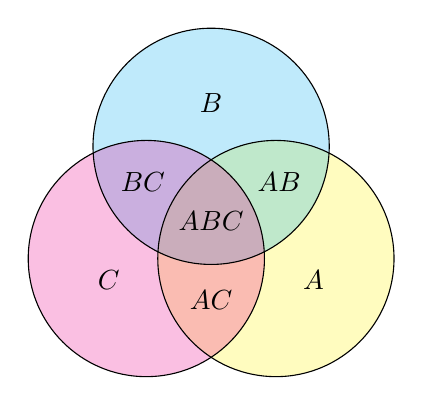
\begin{tikzpicture}
    \begin{scope}[fill opacity=0.25]

        \fill[yellow] \circleA;
        \fill[cyan] \circleB;
        \fill[magenta] \circleC;
        \draw \circleA;
        \draw \circleB;
        \draw \circleC;
    \end{scope}
    \node at (\angA:\doutertext) {$A$};
    \node at (\angB:\doutertext) {$B$};
    \node at (\angC:\doutertext) {$C$};
    \node at ({(\angA+\angB-360)/2}:\dinnertext) {$AB$};
    \node at ({(\angB+\angC)/2}:\dinnertext) {$BC$};
    \node at ({(\angA+\angC)/2}:\dinnertext) {$AC$};
    \node at (0,0) {$ABC$};
\end{tikzpicture}